\newpage
\section{Performance of the project Developed (so far)}

\subsection{Blockchain Structure}
\begin{figure}[h]
    \centering
    \includegraphics[scale=0.45]{images/blockchain.png}\\[0.5cm]
    \caption{Blockchain Structure}
    \label{fig:blockchain}
\end{figure}

\subsection{User Interface}
% It has a feature of uploading transcripts on the blockchain, viewing transcripts
\begin{itemize}
    \item Admin Login
    \item User Login
    \item Dashboard
    \begin{itemize}
        \item Upload transcripts
        \item Access transcripts
    \end{itemize}
    \item Admin access to Blockchain
    \item Admin access to add a new block in the Blockchain
\end{itemize}

\subsection{IPFS}
IPFS i.e. Interplanetary File System is a peer-to-peer protocol where each node stores a collection of hashed files. A client who wants to retrieve any of those files enjoys access to a nice abstraction layer where it simply needs to call the hash of the file it wants. IPFS then combs through the nodes and supplies the client with the file.
It is a decentralized way of storing and referring to files but gives you more control and refers to files by hashes, allowing for much richer programmatic interactions.

\noindent
\\
\textbf{Implementation of IPFS with blockchain:}

\noindent
\\
\textbf{IPFS Workflow:}
\begin{figure}[h]
    \centering
    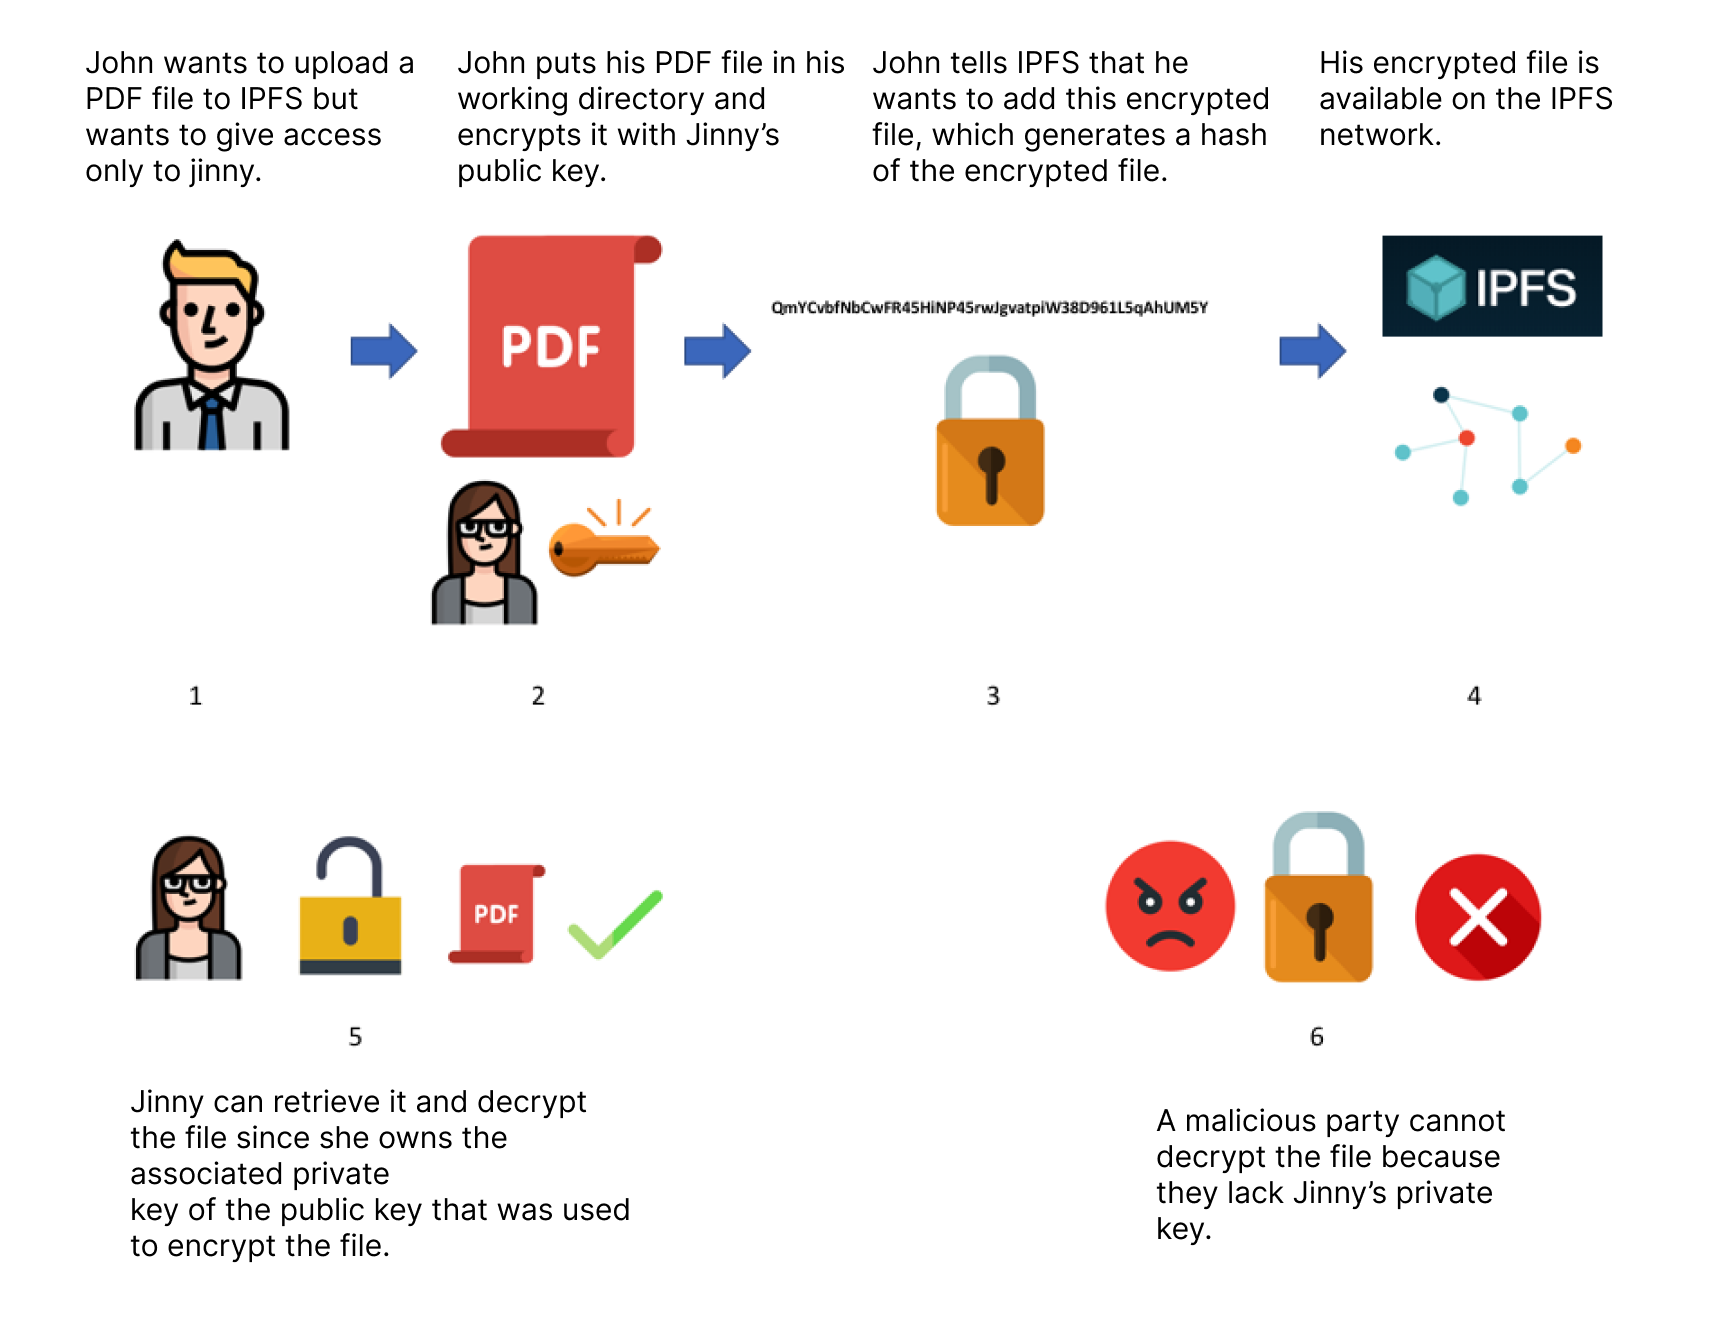
\includegraphics[scale=0.45]{images/ipfs_workflow.png}\\[0.5cm]
    \caption{IPFS Workflow}
    \label{fig:ipfs_workflow}
\end{figure}

\begin{enumerate}
    \item John wants to Upload file on IPFS.
    \item He encrypted it with Jinny's public key.
    \item He uploaded it onto the IPFS.
    \item File is available on the IPFS network.
    \item Jinny can access that file with her private key.
    \item No one else can decrypt the file.
\end{enumerate}

% \clearpage
\noindent
\textbf{Integration of IPFS with Blockchain:}
\begin{figure}[!h]
    \centering
    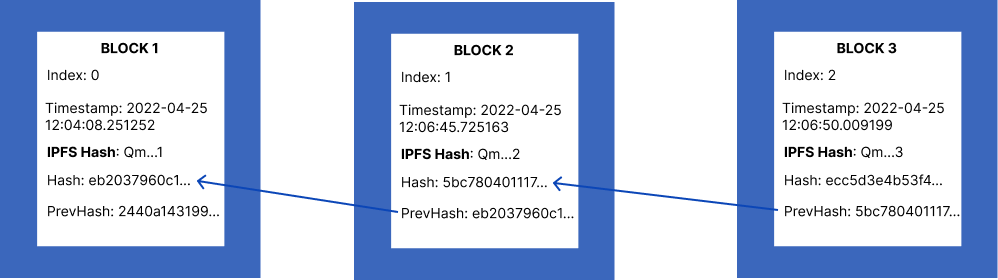
\includegraphics[scale=0.4]{images/ipfs_blockchain.png}\\[0.5cm]
    \caption{Integration of IPFS with Blockchain}
    \label{fig:ipfs_workflow}
\end{figure}

\noindent
In blocks of Blockchain, we simply store the hash of the IPFS file. Thus, we have a very elegant way of storing, encrypting, and sharing large data and files on the blockchain.